\documentclass[11pt,a4paper]{article}
\usepackage{isabelle,isabellesym,amsmath,amssymb,a4wide}
\usepackage{graphicx,xcolor}

\newcommand{\imp}{\rightarrow}
\newcommand{\biimp}{\leftrightarrow}
\newcommand{\all}{\forall}
\newcommand{\ex}{\exists}
\newcommand{\seq}{\vdash}
\newcommand{\nec}{\Box} % necessarily
\newcommand{\pos}{\Diamond} % possibly
\newcommand{\ess}[2]{#1 \ \mathit{ess.} \ #2}
\newcommand{\NE}{\mathit{NE}}


% further packages required for unusual symbols (see also
% isabellesym.sty), use only when needed

%\usepackage{amssymb}
  %for \<leadsto>, \<box>, \<diamond>, \<sqsupset>, \<mho>, \<Join>,
  %\<lhd>, \<lesssim>, \<greatersim>, \<lessapprox>, \<greaterapprox>,
  %\<triangleq>, \<yen>, \<lozenge>

%\usepackage{eurosym}
  %for \<euro>

%\usepackage[only,bigsqcap]{stmaryrd}
  %for \<Sqinter>

%\usepackage{eufrak}
  %for \<AA> ... \<ZZ>, \<aa> ... \<zz> (also included in amssymb)

%\usepackage{textcomp}
  %for \<onequarter>, \<onehalf>, \<threequarters>, \<degree>, \<cent>,
  %\<currency>

% this should be the last package used
\usepackage{pdfsetup}

% urls in roman style, theory text in math-similar italics
\urlstyle{rm}
\isabellestyle{it}

% for uniform font size
%\renewcommand{\isastyle}{\isastyleminor}


\begin{document}

\title{G\"odel's God in Isabelle/HOL}
\author{Christoph Benzm\"uller and Bruno Woltzenlogel Paleo}
%\date{November 1, 2013}
\maketitle

%\noindent\colorbox{gray}{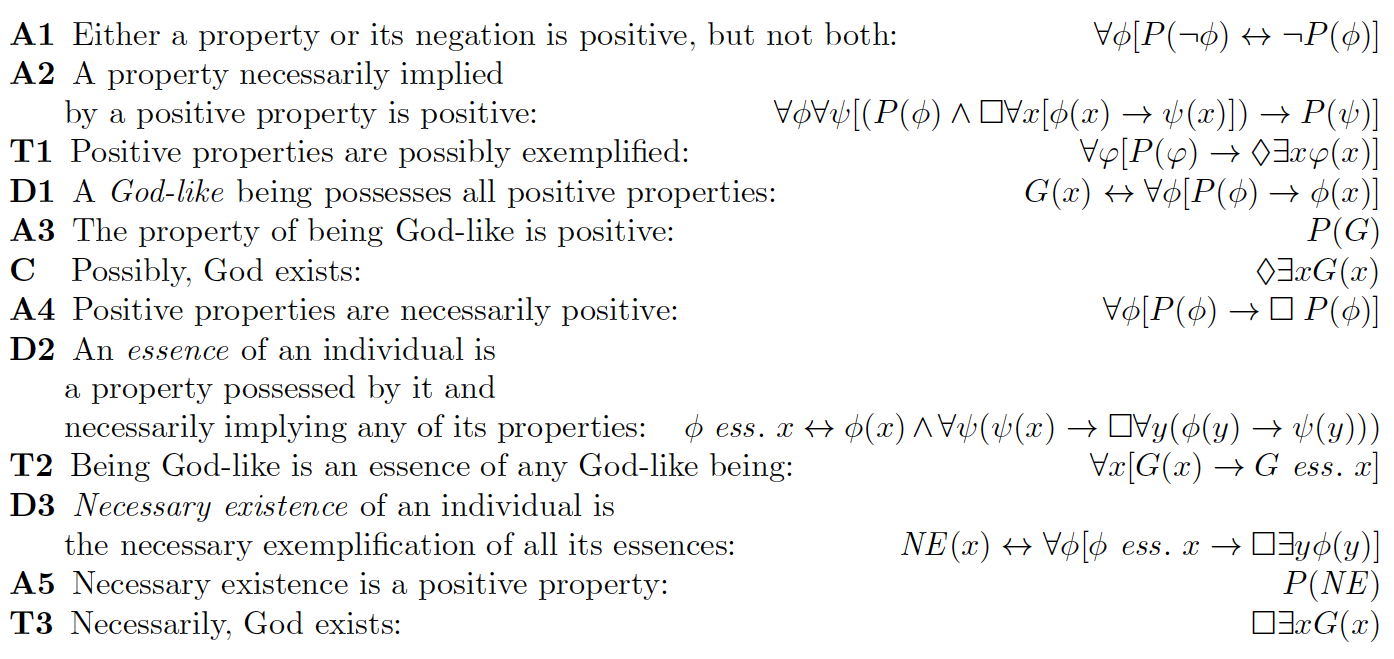
\includegraphics[width=.99\textwidth]{$HOME/GoedelGod/Talks/FU-Berlin/ScottsScriptGrab}} %$

\begin{figure}[h]
\noindent\fcolorbox{gray}{white}{
\begin{minipage}{.96\textwidth}\small
\begin{itemize}
\item[A1] Either a property or its negation is positive, but not
  both:  \hfill 
  $\all \phi [P(\neg \phi) \biimp \neg P(\phi)]$ \\[-1.5em]
\item[A2] A property necessarily implied \\ by a
  positive property is positive: \phantom{b} \hfill 
  $\all \phi \all \psi [(P(\phi) \wedge \nec \all x [\phi(x)
  \imp \psi(x)]) \imp P(\psi)]$ \\[-1.5em]
\item[T1] Positive properties are possibly exemplified: \hfill $\all
  \phi [P(\phi) \imp \pos \ex x \phi(x)]$ \\[-1.5em]
\item[D1] A \emph{God-like} being possesses all positive properties: \hfill
  $G(x) \biimp \forall \phi [P(\phi) \to \phi(x)]$ \\[-1.5em]
\item[A3]  The property of being God-like is positive: \hfill   $P(G)$ \\[-1.5em]
\item[C\phantom{1}] Possibly, God exists: \hfill $\pos \ex x G(x)$ \\[-1.5em]
\item[A4]  Positive properties are necessarily positive: \hfill 
  $\all \phi [P(\phi) \to \Box \; P(\phi)]$ \\[-1.5em]
\item[D2] An \emph{essence} of an individual is a property possessed by it \\ and necessarily implying any of its properties: \\
  \phantom{b} \hfill $\ess{\phi}{x} \biimp \phi(x) \wedge \all
  \psi (\psi(x) \imp \nec \all y (\phi(y) \imp \psi(y)))$ \\[-1.5em]
\item[T2]  Being God-like is an essence of any
  God-like being: \hfill $\all x [G(x) \imp \ess{G}{x}]$ \\[-1.5em]
\item[D3] \emph{Necessary existence} of an individual is \\ the necessary exemplification of all its essences: 
  \phantom{b} \hfill $\NE(x) \biimp \all \phi [\ess{\phi}{x} \imp \nec
  \ex y \phi(y)]$ \\[-1.5em]
\item[A5] Necessary existence is a positive property: \hfill $P(\NE)$ \\[-1.5em]
\item[T3] Necessarily, God exists: \hfill $\nec \ex x G(x)$ 
\end{itemize}
\end{minipage}
}
\caption{Scott's version of G\"odel's ontological argument \cite{ScottNotes}.} 
\end{figure}
\vskip1em

%\tableofcontents

% sane default for proof documents
\parindent 0pt\parskip 0.5ex

% generated text of all theories
%
\begin{isabellebody}%
\def\isabellecontext{GoedelGod}%
%
\isadelimtheory
%
\endisadelimtheory
%
\isatagtheory
%
\endisatagtheory
{\isafoldtheory}%
%
\isadelimtheory
%
\endisadelimtheory
%
\isamarkupsection{Introduction%
}
\isamarkuptrue%
%
\begin{isamarkuptext}%
Dana Scott's version \cite{ScottNotes}
 of Goedel's ontological argument \cite{GoedelNotes} is 
 formalized in quantified modal logic KB (QML KB) within the proof assistant Isabelle/HOL. 
 QML KB is  modeled as a fragment of classical higher-order logic (HOL); 
 thus, the formalization is essentially a formalization in HOL. The employed embedding 
 of QML KB in HOL is adapting the work of Benzm\"uller and Paulson \cite{J23,B9}.
 Note that the QML KB formalization employs quantification over individuals and 
 quantification over sets of individuals (properties).

 The gaps in Scott's proof have been automated 
 with Sledgehammer \cite{Sledgehammer}, performing remote calls to the higher-order automated
 theorem prover LEO-II \cite{LEO-II}. Sledgehammer then suggests the 
 Metis \cite{Metis} calls. The Metis proofs are verified by Isabelle/HOL.
 For consistency checking, the model finder Nitpick \cite{Nitpick} has been employed.
 The successfull calls to Sledgehammer (normally, they automatically eliminated by Isabelle/HOL)
 are deliberately kept in the file for demonstration purposes.
 
 Isabelle is described in the textbook by Nipkow, 
 Paulson, and Wenzel \cite{Isabelle} and in tutorials available 
 at: \url{http://isabelle.in.tum.de}.
 
\subsection{Related Work}

 The formalization presented here is related to the THF \cite{J22} and 
 Coq \cite{Coq} formalizations at 
 \url{https://github.com/FormalTheology/GoedelGod/tree/master/Formalizations/}.
 
 An older ontological argument by Anselm was formalized in PVS by John Rushby \cite{rushby}.%
\end{isamarkuptext}%
\isamarkuptrue%
%
\isamarkupsection{An Embedding of QML KB in HOL%
}
\isamarkuptrue%
%
\begin{isamarkuptext}%
The types \isa{i} for possible worlds and $\mu$ for individuals 
are introduced.%
\end{isamarkuptext}%
\isamarkuptrue%
\ \ \isacommand{typedecl}\isamarkupfalse%
\ i\ \ \ \ %
\isamarkupcmt{the type for possible worlds%
}
\ \isanewline
\ \ \isacommand{typedecl}\isamarkupfalse%
\ {\isasymmu}\ \ \ \ %
\isamarkupcmt{the type for indiviuals%
}
%
\begin{isamarkuptext}%
Possible worlds are connected by an accessibility relation \isa{r}.%
\end{isamarkuptext}%
\isamarkuptrue%
\ \ \isacommand{consts}\isamarkupfalse%
\ r\ {\isacharcolon}{\isacharcolon}\ {\isachardoublequoteopen}i\ {\isasymRightarrow}\ i\ {\isasymRightarrow}\ bool{\isachardoublequoteclose}\ {\isacharparenleft}\isakeyword{infixr}\ {\isachardoublequoteopen}r{\isachardoublequoteclose}\ {\isadigit{7}}{\isadigit{0}}{\isacharparenright}\ \ \ \ %
\isamarkupcmt{accessibility relation r%
}
%
\begin{isamarkuptext}%
QML formulas are translated as HOL terms of type \isa{i\ {\isasymRightarrow}\ bool}. 
This type is abbreviated as \isa{{\isasymsigma}}.%
\end{isamarkuptext}%
\isamarkuptrue%
\ \ \isacommand{type{\isacharunderscore}synonym}\isamarkupfalse%
\ {\isasymsigma}\ {\isacharequal}\ {\isachardoublequoteopen}{\isacharparenleft}i\ {\isasymRightarrow}\ bool{\isacharparenright}{\isachardoublequoteclose}%
\begin{isamarkuptext}%
The classical connectives $\neg, \wedge, \rightarrow$, and $\forall$
(over individuals and over sets of individuals) and $\exists$ (over individuals) are
lifted to type $\sigma$. The lifted connectives are \isa{m{\isasymnot}}, \isa{m{\isasymand}}, \isa{m{\isasymrightarrow}},
\isa{{\isasymforall}}, and \isa{{\isasymexists}} (the latter two are modeled as constant symbols). 
Other connectives can be introduced analogously. We exemplarily do this for $\vee$, 
$\leftrightarrow$, and $=$. Moreover, the modal operators $\Box$ and $\diamond$ are introduced.
Definitions could be used instead of abbreviations.%
\end{isamarkuptext}%
\isamarkuptrue%
\ \ \isacommand{abbreviation}\isamarkupfalse%
\ mnot\ {\isacharcolon}{\isacharcolon}\ {\isachardoublequoteopen}{\isasymsigma}\ {\isasymRightarrow}\ {\isasymsigma}{\isachardoublequoteclose}\ {\isacharparenleft}{\isachardoublequoteopen}m{\isasymnot}{\isachardoublequoteclose}{\isacharparenright}\ \isakeyword{where}\ {\isachardoublequoteopen}m{\isasymnot}\ {\isasymphi}\ {\isasymequiv}\ {\isacharparenleft}{\isasymlambda}w{\isachardot}\ {\isasymnot}\ {\isasymphi}\ w{\isacharparenright}{\isachardoublequoteclose}\ \ \ \ \isanewline
\ \ \isacommand{abbreviation}\isamarkupfalse%
\ mand\ {\isacharcolon}{\isacharcolon}\ {\isachardoublequoteopen}{\isasymsigma}\ {\isasymRightarrow}\ {\isasymsigma}\ {\isasymRightarrow}\ {\isasymsigma}{\isachardoublequoteclose}\ {\isacharparenleft}\isakeyword{infixr}\ {\isachardoublequoteopen}m{\isasymand}{\isachardoublequoteclose}\ {\isadigit{6}}{\isadigit{5}}{\isacharparenright}\ \isakeyword{where}\ {\isachardoublequoteopen}{\isasymphi}\ m{\isasymand}\ {\isasympsi}\ {\isasymequiv}\ {\isacharparenleft}{\isasymlambda}w{\isachardot}\ {\isasymphi}\ w\ {\isasymand}\ {\isasympsi}\ w{\isacharparenright}{\isachardoublequoteclose}\ \ \ \isanewline
\ \ \isacommand{abbreviation}\isamarkupfalse%
\ mor\ {\isacharcolon}{\isacharcolon}\ {\isachardoublequoteopen}{\isasymsigma}\ {\isasymRightarrow}\ {\isasymsigma}\ {\isasymRightarrow}\ {\isasymsigma}{\isachardoublequoteclose}\ {\isacharparenleft}\isakeyword{infixr}\ {\isachardoublequoteopen}m{\isasymor}{\isachardoublequoteclose}\ {\isadigit{7}}{\isadigit{0}}{\isacharparenright}\ \isakeyword{where}\ {\isachardoublequoteopen}{\isasymphi}\ m{\isasymor}\ {\isasympsi}\ {\isasymequiv}\ {\isacharparenleft}{\isasymlambda}w{\isachardot}\ {\isasymphi}\ w\ {\isasymor}\ {\isasympsi}\ w{\isacharparenright}{\isachardoublequoteclose}\ \ \ \isanewline
\ \ \isacommand{abbreviation}\isamarkupfalse%
\ mimplies\ {\isacharcolon}{\isacharcolon}\ {\isachardoublequoteopen}{\isasymsigma}\ {\isasymRightarrow}\ {\isasymsigma}\ {\isasymRightarrow}\ {\isasymsigma}{\isachardoublequoteclose}\ {\isacharparenleft}\isakeyword{infixr}\ {\isachardoublequoteopen}m{\isasymrightarrow}{\isachardoublequoteclose}\ {\isadigit{7}}{\isadigit{4}}{\isacharparenright}\ \isakeyword{where}\ {\isachardoublequoteopen}{\isasymphi}\ m{\isasymrightarrow}\ {\isasympsi}\ {\isasymequiv}\ {\isacharparenleft}{\isasymlambda}w{\isachardot}\ {\isasymphi}\ w\ {\isasymlongrightarrow}\ {\isasympsi}\ w{\isacharparenright}{\isachardoublequoteclose}\ \ \isanewline
\ \ \isacommand{abbreviation}\isamarkupfalse%
\ mequiv{\isacharcolon}{\isacharcolon}\ {\isachardoublequoteopen}{\isasymsigma}\ {\isasymRightarrow}\ {\isasymsigma}\ {\isasymRightarrow}\ {\isasymsigma}{\isachardoublequoteclose}\ {\isacharparenleft}\isakeyword{infixr}\ {\isachardoublequoteopen}m{\isasymequiv}{\isachardoublequoteclose}\ {\isadigit{7}}{\isadigit{6}}{\isacharparenright}\ \isakeyword{where}\ {\isachardoublequoteopen}{\isasymphi}\ m{\isasymequiv}\ {\isasympsi}\ {\isasymequiv}\ {\isacharparenleft}{\isasymlambda}w{\isachardot}\ {\isacharparenleft}{\isasymphi}\ w\ {\isasymlongleftrightarrow}\ {\isasympsi}\ w{\isacharparenright}{\isacharparenright}{\isachardoublequoteclose}\ \ \isanewline
\ \ \isacommand{abbreviation}\isamarkupfalse%
\ meq\ {\isacharcolon}{\isacharcolon}\ {\isachardoublequoteopen}{\isacharprime}a\ {\isasymRightarrow}\ {\isacharprime}a\ {\isasymRightarrow}\ {\isasymsigma}{\isachardoublequoteclose}\ {\isacharparenleft}\isakeyword{infixr}\ {\isachardoublequoteopen}m{\isacharequal}{\isachardoublequoteclose}\ {\isadigit{5}}{\isadigit{0}}{\isacharparenright}\ \isakeyword{where}\ {\isachardoublequoteopen}x\ m{\isacharequal}\ y\ {\isasymequiv}\ {\isacharparenleft}{\isasymlambda}w{\isachardot}\ x\ {\isacharequal}\ y{\isacharparenright}{\isachardoublequoteclose}\isanewline
\ \ \isacommand{abbreviation}\isamarkupfalse%
\ mforall\ {\isacharcolon}{\isacharcolon}\ {\isachardoublequoteopen}{\isacharparenleft}{\isacharprime}a\ {\isasymRightarrow}\ {\isasymsigma}{\isacharparenright}\ {\isasymRightarrow}\ {\isasymsigma}{\isachardoublequoteclose}\ {\isacharparenleft}{\isachardoublequoteopen}{\isasymforall}{\isachardoublequoteclose}{\isacharparenright}\ \isakeyword{where}\ {\isachardoublequoteopen}{\isasymforall}\ {\isasymPhi}\ {\isasymequiv}\ {\isacharparenleft}{\isasymlambda}w{\isachardot}\ {\isasymforall}x{\isachardot}\ {\isasymPhi}\ x\ w{\isacharparenright}{\isachardoublequoteclose}\ \ \ \isanewline
\ \ \isacommand{abbreviation}\isamarkupfalse%
\ mexists\ {\isacharcolon}{\isacharcolon}\ {\isachardoublequoteopen}{\isacharparenleft}{\isacharprime}a\ {\isasymRightarrow}\ {\isasymsigma}{\isacharparenright}\ {\isasymRightarrow}\ {\isasymsigma}{\isachardoublequoteclose}\ {\isacharparenleft}{\isachardoublequoteopen}{\isasymexists}{\isachardoublequoteclose}{\isacharparenright}\ \isakeyword{where}\ {\isachardoublequoteopen}{\isasymexists}\ {\isasymPhi}\ {\isasymequiv}\ {\isacharparenleft}{\isasymlambda}w{\isachardot}\ {\isasymexists}x{\isachardot}\ {\isasymPhi}\ x\ w{\isacharparenright}{\isachardoublequoteclose}\isanewline
\ \ \isacommand{abbreviation}\isamarkupfalse%
\ mbox\ {\isacharcolon}{\isacharcolon}\ {\isachardoublequoteopen}{\isasymsigma}\ {\isasymRightarrow}\ {\isasymsigma}{\isachardoublequoteclose}\ {\isacharparenleft}{\isachardoublequoteopen}{\isasymbox}{\isachardoublequoteclose}{\isacharparenright}\ \isakeyword{where}\ {\isachardoublequoteopen}{\isasymbox}\ {\isasymphi}\ {\isasymequiv}\ {\isacharparenleft}{\isasymlambda}w{\isachardot}\ {\isasymforall}v{\isachardot}\ \ w\ r\ v\ {\isasymlongrightarrow}\ {\isasymphi}\ v{\isacharparenright}{\isachardoublequoteclose}\isanewline
\ \ \isacommand{abbreviation}\isamarkupfalse%
\ mdia\ {\isacharcolon}{\isacharcolon}\ {\isachardoublequoteopen}{\isasymsigma}\ {\isasymRightarrow}\ {\isasymsigma}{\isachardoublequoteclose}\ {\isacharparenleft}{\isachardoublequoteopen}{\isasymdiamond}{\isachardoublequoteclose}{\isacharparenright}\ \isakeyword{where}\ {\isachardoublequoteopen}{\isasymdiamond}\ {\isasymphi}\ {\isasymequiv}\ {\isacharparenleft}{\isasymlambda}w{\isachardot}\ {\isasymexists}v{\isachardot}\ w\ r\ v\ {\isasymand}\ {\isasymphi}\ v{\isacharparenright}{\isachardoublequoteclose}%
\begin{isamarkuptext}%
For grounding lifted formulas, the meta-predicate \isa{valid} is introduced.%
\end{isamarkuptext}%
\isamarkuptrue%
\ \ \isacommand{abbreviation}\isamarkupfalse%
\ valid\ {\isacharcolon}{\isacharcolon}\ {\isachardoublequoteopen}{\isasymsigma}\ {\isasymRightarrow}\ bool{\isachardoublequoteclose}\ {\isacharparenleft}{\isachardoublequoteopen}{\isacharbrackleft}{\isacharunderscore}{\isacharbrackright}{\isachardoublequoteclose}{\isacharparenright}\ \isakeyword{where}\ {\isachardoublequoteopen}{\isacharbrackleft}p{\isacharbrackright}\ {\isasymequiv}\ {\isasymforall}w{\isachardot}\ p\ w{\isachardoublequoteclose}%
\isamarkupsection{G\"odel's Ontological Argument%
}
\isamarkuptrue%
%
\begin{isamarkuptext}%
Constant symbol \isa{P} (G\"odel's `Positive') is declared.%
\end{isamarkuptext}%
\isamarkuptrue%
\ \ \isacommand{consts}\isamarkupfalse%
\ P\ {\isacharcolon}{\isacharcolon}\ {\isachardoublequoteopen}{\isacharparenleft}{\isasymmu}\ {\isasymRightarrow}\ {\isasymsigma}{\isacharparenright}\ {\isasymRightarrow}\ {\isasymsigma}{\isachardoublequoteclose}%
\begin{isamarkuptext}%
The meaning of \isa{P} is restricted by axioms \isa{A{\isadigit{1}}{\isacharparenleft}a{\isacharslash}b{\isacharparenright}}: $\all \varphi 
[P(\neg \varphi) \biimp \neg P(\varphi)]$ (Either a property or its negation is positive, but not both.) 
and \isa{A{\isadigit{2}}}: $\all \varphi \all \psi [(P(\varphi) \wedge \nec \all x [\varphi(x) \imp \psi(x)]) 
\imp P(\psi)]$ (A property necessarily implied by a positive property is positive).%
\end{isamarkuptext}%
\isamarkuptrue%
\ \ \isacommand{axiomatization}\isamarkupfalse%
\ \isakeyword{where}\isanewline
\ \ \ \ A{\isadigit{1}}a{\isacharcolon}\ {\isachardoublequoteopen}{\isacharbrackleft}{\isasymforall}{\isacharparenleft}{\isasymlambda}{\isasymphi}{\isachardot}\ P\ {\isacharparenleft}{\isasymlambda}x{\isachardot}\ m{\isasymnot}\ {\isacharparenleft}{\isasymphi}\ x{\isacharparenright}{\isacharparenright}\ m{\isasymrightarrow}\ m{\isasymnot}\ {\isacharparenleft}P\ {\isasymphi}{\isacharparenright}{\isacharparenright}{\isacharbrackright}{\isachardoublequoteclose}\ \isakeyword{and}\isanewline
\ \ \ \ A{\isadigit{1}}b{\isacharcolon}\ {\isachardoublequoteopen}{\isacharbrackleft}{\isasymforall}{\isacharparenleft}{\isasymlambda}{\isasymphi}{\isachardot}\ m{\isasymnot}\ {\isacharparenleft}P\ {\isasymphi}{\isacharparenright}\ m{\isasymrightarrow}\ P\ {\isacharparenleft}{\isasymlambda}x{\isachardot}\ m{\isasymnot}\ {\isacharparenleft}{\isasymphi}\ x{\isacharparenright}{\isacharparenright}{\isacharparenright}{\isacharbrackright}{\isachardoublequoteclose}\ \isakeyword{and}\isanewline
\ \ \ \ A{\isadigit{2}}{\isacharcolon}\ \ {\isachardoublequoteopen}{\isacharbrackleft}{\isasymforall}{\isacharparenleft}{\isasymlambda}{\isasymphi}{\isachardot}\ {\isasymforall}{\isacharparenleft}{\isasymlambda}{\isasympsi}{\isachardot}\ {\isacharparenleft}P\ {\isasymphi}\ m{\isasymand}\ {\isasymbox}\ {\isacharparenleft}{\isasymforall}{\isacharparenleft}{\isasymlambda}x{\isachardot}\ {\isasymphi}\ x\ m{\isasymrightarrow}\ {\isasympsi}\ x{\isacharparenright}{\isacharparenright}{\isacharparenright}\ m{\isasymrightarrow}\ P\ {\isasympsi}{\isacharparenright}{\isacharparenright}{\isacharbrackright}{\isachardoublequoteclose}%
\begin{isamarkuptext}%
We prove theorem T1: $\all \varphi [P(\varphi) \imp \pos \ex x \varphi(x)]$ (Positive 
properties are possibly exemplified). T1 is proved directly by Sledgehammer with command \isa{sledgehammer\ {\isacharbrackleft}provers\ {\isacharequal}\ remote{\isacharunderscore}leo{\isadigit{2}}{\isacharbrackright}}. 
Sledgehammer suggests to call Metis with axioms A1a and A2. 
Metis sucesfully generates a proof object 
that is verified in Isabelle/HOL's kernel.%
\end{isamarkuptext}%
\isamarkuptrue%
\ \ \isacommand{theorem}\isamarkupfalse%
\ T{\isadigit{1}}{\isacharcolon}\ {\isachardoublequoteopen}{\isacharbrackleft}{\isasymforall}{\isacharparenleft}{\isasymlambda}{\isasymphi}{\isachardot}\ P\ {\isasymphi}\ m{\isasymrightarrow}\ {\isasymdiamond}\ {\isacharparenleft}{\isasymexists}\ {\isasymphi}{\isacharparenright}{\isacharparenright}{\isacharbrackright}{\isachardoublequoteclose}\ \ \isanewline
\ \ \isacommand{sledgehammer}\isamarkupfalse%
\ {\isacharbrackleft}provers\ {\isacharequal}\ remote{\isacharunderscore}leo{\isadigit{2}}{\isacharbrackright}\ \isanewline
%
\isadelimproof
\ \ %
\endisadelimproof
%
\isatagproof
\isacommand{by}\isamarkupfalse%
\ {\isacharparenleft}metis\ A{\isadigit{1}}a\ A{\isadigit{2}}{\isacharparenright}%
\endisatagproof
{\isafoldproof}%
%
\isadelimproof
%
\endisadelimproof
%
\begin{isamarkuptext}%
Next, the symbol \isa{G} for `God-like'  is introduced and defined 
as $G(x) \biimp \forall \varphi [P(\phi) \to \varphi(x)]$ \\ (A God-like being possesses 
all positive properties).%
\end{isamarkuptext}%
\isamarkuptrue%
\ \ \isacommand{definition}\isamarkupfalse%
\ G\ {\isacharcolon}{\isacharcolon}\ {\isachardoublequoteopen}{\isasymmu}\ {\isasymRightarrow}\ {\isasymsigma}{\isachardoublequoteclose}\ \isakeyword{where}\ {\isachardoublequoteopen}G\ {\isacharequal}\ {\isacharparenleft}{\isasymlambda}x{\isachardot}\ {\isasymforall}{\isacharparenleft}{\isasymlambda}{\isasymphi}{\isachardot}\ P\ {\isasymphi}\ m{\isasymrightarrow}\ {\isasymphi}\ x{\isacharparenright}{\isacharparenright}{\isachardoublequoteclose}%
\begin{isamarkuptext}%
Axiom \isa{A{\isadigit{3}}} is added: $P(G)$ (The property of being God-like is positive).
Sledgehammer and Metis then prove corollary \isa{C}: $\pos \ex x G(x)$ 
(Possibly, God exists).%
\end{isamarkuptext}%
\isamarkuptrue%
\ \ \isacommand{axiomatization}\isamarkupfalse%
\ \isakeyword{where}\ A{\isadigit{3}}{\isacharcolon}\ \ {\isachardoublequoteopen}{\isacharbrackleft}P\ G{\isacharbrackright}{\isachardoublequoteclose}\ \isanewline
\isanewline
\ \ \isacommand{corollary}\isamarkupfalse%
\ C{\isacharcolon}\ {\isachardoublequoteopen}{\isacharbrackleft}{\isasymdiamond}\ {\isacharparenleft}{\isasymexists}\ G{\isacharparenright}{\isacharbrackright}{\isachardoublequoteclose}\ \isanewline
\ \ \isacommand{sledgehammer}\isamarkupfalse%
\ {\isacharbrackleft}provers\ {\isacharequal}\ remote{\isacharunderscore}leo{\isadigit{2}}{\isacharbrackright}\ \isanewline
%
\isadelimproof
\ \ %
\endisadelimproof
%
\isatagproof
\isacommand{by}\isamarkupfalse%
\ {\isacharparenleft}metis\ A{\isadigit{3}}\ T{\isadigit{1}}{\isacharparenright}%
\endisatagproof
{\isafoldproof}%
%
\isadelimproof
%
\endisadelimproof
%
\begin{isamarkuptext}%
Axiom \isa{A{\isadigit{4}}} is added: $\all \phi [P(\phi) \to \Box \; P(\phi)]$ 
(Positive properties are necessarily positive).%
\end{isamarkuptext}%
\isamarkuptrue%
\ \ \isacommand{axiomatization}\isamarkupfalse%
\ \isakeyword{where}\ A{\isadigit{4}}{\isacharcolon}\ \ {\isachardoublequoteopen}{\isacharbrackleft}{\isasymforall}{\isacharparenleft}{\isasymlambda}{\isasymphi}{\isachardot}\ P\ {\isasymphi}\ m{\isasymrightarrow}\ {\isasymbox}\ {\isacharparenleft}P\ {\isasymphi}{\isacharparenright}{\isacharparenright}{\isacharbrackright}{\isachardoublequoteclose}%
\begin{isamarkuptext}%
Symbol \isa{ess} for `Essence' is introduced and defined as 
$$\ess{\varphi}{x} \biimp \varphi(x) \wedge \all \psi (\psi(x) \imp \nec \all y (\varphi(y) 
\imp \psi(y)))$$ (An \emph{essence} of an individual is a property possessed by it and necessarily implying any of its properties).%
\end{isamarkuptext}%
\isamarkuptrue%
\ \ \isacommand{definition}\isamarkupfalse%
\ ess\ {\isacharcolon}{\isacharcolon}\ {\isachardoublequoteopen}{\isacharparenleft}{\isasymmu}\ {\isasymRightarrow}\ {\isasymsigma}{\isacharparenright}\ {\isasymRightarrow}\ {\isasymmu}\ {\isasymRightarrow}\ {\isasymsigma}{\isachardoublequoteclose}\ {\isacharparenleft}\isakeyword{infixr}\ {\isachardoublequoteopen}ess{\isachardoublequoteclose}\ {\isadigit{8}}{\isadigit{5}}{\isacharparenright}\ \isakeyword{where}\isanewline
\ \ \ \ {\isachardoublequoteopen}{\isasymphi}\ ess\ x\ {\isacharequal}\ {\isasymphi}\ x\ m{\isasymand}\ {\isasymforall}{\isacharparenleft}{\isasymlambda}{\isasympsi}{\isachardot}\ {\isasympsi}\ x\ m{\isasymrightarrow}\ {\isasymbox}\ {\isacharparenleft}{\isasymforall}{\isacharparenleft}{\isasymlambda}y{\isachardot}\ {\isasymphi}\ y\ m{\isasymrightarrow}\ {\isasympsi}\ y{\isacharparenright}{\isacharparenright}{\isacharparenright}{\isachardoublequoteclose}%
\begin{isamarkuptext}%
Next, Sledgehammer and Metis prove theorem \isa{T{\isadigit{2}}}: $\all x [G(x) \imp \ess{G}{x}]$ \\
(Being God-like is an essence of any God-like being).%
\end{isamarkuptext}%
\isamarkuptrue%
\ \ \isacommand{theorem}\isamarkupfalse%
\ T{\isadigit{2}}{\isacharcolon}\ {\isachardoublequoteopen}{\isacharbrackleft}{\isasymforall}{\isacharparenleft}{\isasymlambda}x{\isachardot}\ G\ x\ m{\isasymrightarrow}\ G\ ess\ x{\isacharparenright}{\isacharbrackright}{\isachardoublequoteclose}\isanewline
\ \ \isacommand{sledgehammer}\isamarkupfalse%
\ {\isacharbrackleft}provers\ {\isacharequal}\ remote{\isacharunderscore}leo{\isadigit{2}}{\isacharbrackright}\ \isanewline
%
\isadelimproof
\ \ %
\endisadelimproof
%
\isatagproof
\isacommand{by}\isamarkupfalse%
\ {\isacharparenleft}metis\ A{\isadigit{1}}b\ A{\isadigit{4}}\ G{\isacharunderscore}def\ ess{\isacharunderscore}def{\isacharparenright}%
\endisatagproof
{\isafoldproof}%
%
\isadelimproof
%
\endisadelimproof
%
\begin{isamarkuptext}%
Symbol \isa{NE}, for `Necessary Existence', is introduced and
defined as $$\NE(x) \biimp \all \varphi [\ess{\varphi}{x} \imp \nec \ex y \varphi(y)]$$ (Necessary 
existence of an individual is the necessary exemplification of all its essences).%
\end{isamarkuptext}%
\isamarkuptrue%
\ \ \isacommand{definition}\isamarkupfalse%
\ NE\ {\isacharcolon}{\isacharcolon}\ {\isachardoublequoteopen}{\isasymmu}\ {\isasymRightarrow}\ {\isasymsigma}{\isachardoublequoteclose}\ \isakeyword{where}\ {\isachardoublequoteopen}NE\ {\isacharequal}\ {\isacharparenleft}{\isasymlambda}x{\isachardot}\ {\isasymforall}{\isacharparenleft}{\isasymlambda}{\isasymphi}{\isachardot}\ {\isasymphi}\ ess\ x\ m{\isasymrightarrow}\ {\isasymbox}\ {\isacharparenleft}{\isasymexists}\ {\isasymphi}{\isacharparenright}{\isacharparenright}{\isacharparenright}{\isachardoublequoteclose}%
\begin{isamarkuptext}%
Moreover, axiom \isa{A{\isadigit{5}}} is added: $P(\NE)$ (Necessary existence is a positive 
property).%
\end{isamarkuptext}%
\isamarkuptrue%
\ \ \isacommand{axiomatization}\isamarkupfalse%
\ \isakeyword{where}\ A{\isadigit{5}}{\isacharcolon}\ \ {\isachardoublequoteopen}{\isacharbrackleft}P\ NE{\isacharbrackright}{\isachardoublequoteclose}%
\begin{isamarkuptext}%
The \isa{B} axiom (symmetry) for relation r is stated. \isa{B} is needed only 
for proving theorem T3 and for corollary C2.%
\end{isamarkuptext}%
\isamarkuptrue%
\ \ \isacommand{axiomatization}\isamarkupfalse%
\ \isakeyword{where}\ sym{\isacharcolon}\ {\isachardoublequoteopen}x\ r\ y\ {\isasymlongrightarrow}\ y\ r\ x{\isachardoublequoteclose}%
\begin{isamarkuptext}%
Finally, Sledgehammer and Metis prove the main theorem \isa{T{\isadigit{3}}}: $\nec \ex x G(x)$ \\
(Necessarily, God exists).%
\end{isamarkuptext}%
\isamarkuptrue%
\ \ \isacommand{theorem}\isamarkupfalse%
\ T{\isadigit{3}}{\isacharcolon}\ {\isachardoublequoteopen}{\isacharbrackleft}{\isasymbox}\ {\isacharparenleft}{\isasymexists}\ G{\isacharparenright}{\isacharbrackright}{\isachardoublequoteclose}\ \isanewline
\ \ \isacommand{sledgehammer}\isamarkupfalse%
\ {\isacharbrackleft}provers\ {\isacharequal}\ remote{\isacharunderscore}leo{\isadigit{2}}{\isacharbrackright}\ \isanewline
%
\isadelimproof
\ \ %
\endisadelimproof
%
\isatagproof
\isacommand{by}\isamarkupfalse%
\ {\isacharparenleft}metis\ A{\isadigit{5}}\ C\ T{\isadigit{2}}\ sym\ G{\isacharunderscore}def\ NE{\isacharunderscore}def{\isacharparenright}%
\endisatagproof
{\isafoldproof}%
%
\isadelimproof
%
\endisadelimproof
%
\begin{isamarkuptext}%
Surprisingly, the following corollary can be derived even without the \isa{T} axiom 
(reflexivity).%
\end{isamarkuptext}%
\isamarkuptrue%
\ \ \isacommand{corollary}\isamarkupfalse%
\ C{\isadigit{2}}{\isacharcolon}\ {\isachardoublequoteopen}{\isacharbrackleft}{\isasymexists}\ G{\isacharbrackright}{\isachardoublequoteclose}\ \isanewline
\ \ \isacommand{sledgehammer}\isamarkupfalse%
\ {\isacharbrackleft}provers\ {\isacharequal}\ remote{\isacharunderscore}leo{\isadigit{2}}{\isacharbrackright}{\isacharparenleft}T{\isadigit{1}}\ T{\isadigit{3}}\ G{\isacharunderscore}def\ sym{\isacharparenright}\ \isanewline
%
\isadelimproof
\ \ %
\endisadelimproof
%
\isatagproof
\isacommand{by}\isamarkupfalse%
\ {\isacharparenleft}metis\ T{\isadigit{1}}\ T{\isadigit{3}}\ G{\isacharunderscore}def\ sym{\isacharparenright}%
\endisatagproof
{\isafoldproof}%
%
\isadelimproof
%
\endisadelimproof
%
\begin{isamarkuptext}%
The consistency of the entire theory is checked with Nitpick.%
\end{isamarkuptext}%
\isamarkuptrue%
\ \ \isacommand{lemma}\isamarkupfalse%
\ True\ \isacommand{nitpick}\isamarkupfalse%
\ {\isacharbrackleft}satisfy{\isacharcomma}\ user{\isacharunderscore}axioms{\isacharcomma}\ expect\ {\isacharequal}\ genuine{\isacharbrackright}%
\isadelimproof
\ %
\endisadelimproof
%
\isatagproof
\isacommand{oops}\isamarkupfalse%
\ \isanewline
%
\endisatagproof
{\isafoldproof}%
%
\isadelimproof
%
\endisadelimproof
%
\isadelimtheory
%
\endisadelimtheory
%
\isatagtheory
%
\endisatagtheory
{\isafoldtheory}%
%
\isadelimtheory
%
\endisadelimtheory
\ \end{isabellebody}%
%%% Local Variables:
%%% mode: latex
%%% TeX-master: "root"
%%% End:


%%% Local Variables:
%%% mode: latex
%%% TeX-master: "root"
%%% End:


% optional bibliography
%\bibliographystyle{abbrv}
%\bibliography{root}

\paragraph{Acknowledgments:} Nik Sultana, Jasmin Blanchette and Larry Paulson provided 
very important help on issues related to consistency checking in Isabelle. Jasmin Blanchette instructed us on 
producing Isabelle sessions and he showed us some useful tricks in Isabelle.

%\small
\begin{thebibliography}{10}

\bibitem{B9}
C.~Benzm{\"u}ller and L.C. Paulson.
\newblock Exploring properties of normal multimodal logics in simple type
  theory with {LEO-II}.
\newblock In {\em {Festschrift in Honor of {Peter B. Andrews} on His 70th
  Birthday}}, pp. 386--406. College Publications.

\bibitem{J23}
C.~Benzm{\"u}ller and L.C. Paulson.
\newblock Quantified multimodal logics in simple type theory.
\newblock {\em Logica Universalis (Special Issue on Multimodal Logics)},
  7(1):7--20, 2013.

\bibitem{LEO-II}
C.~Benzm{\"u}ller, F.~Theiss, L.~Paulson, and A.~Fietzke.
\newblock {LEO-II} - a cooperative automatic theorem prover for higher-order
  logic.
\newblock In {\em Proc. of IJCAR 2008}, volume 5195 of {\em LNAI}, pp.
  162--170. Springer, 2008.

\bibitem{Coq}
Y.~Bertot and P.~Casteran.
\newblock {\em {Interactive Theorem Proving and Program Development}}.
\newblock Springer, 2004.

\bibitem{Sledgehammer}
J.C. Blanchette, S.~B\"ohme, and L.C. Paulson.
\newblock Extending {Sledgehammer} with {SMT} solvers.
\newblock {\em Journal of Automated Reasoning}, 51(1):109--128, 2013.

\bibitem{Nitpick}
J.C. Blanchette and T.~Nipkow.
\newblock Nitpick: A counterexample generator for higher-order logic based on a
  relational model finder.
\newblock In {\em Proc. of ITP 2010}, LNCS 6172, pp. 131--146.
  Springer, 2010.

\bibitem{Satallax}
C.E. Brown.
\newblock Satallax: An automated higher-order prover.
\newblock In {\em Proc. of IJCAR 2012}, LNAI 7364, pp. 111 -- 117.
  Springer, 2012.

\bibitem{GoedelNotes}
K.~G\"odel.
\newblock {\em Appendix A. Notes in Kurt G\"odel's Hand}, pp. 144--145.
\newblock In  \cite{sobel2004logic}, 2004.


\bibitem{Metis}
J.~Hurd.
\newblock First-order proof tactics in higher-order logic theorem provers.
\newblock In {\em Design and Application of Strategies/Tactics in Higher Order
  Logics, NASA Tech. Rep. NASA/CP-2003-212448}, 2003.

\bibitem{Isabelle}
T.~Nipkow, L.C. Paulson, and M.~Wenzel.
\newblock {\em {Isabelle/HOL: A Proof Assistant for Higher-Order Logic}}.
\newblock LNCS 2283. Springer, 2002.

\bibitem{rushby}
J.~Rushby.
\newblock The Ontological Argument in PVS. 
\newblock {\em CAV Workshop ``Fun With Formal Methods'}, St. Petersburg, Russia, 13th of July 2013.

\bibitem{ScottNotes}
D.~Scott.
\newblock {\em Appendix B. Notes in Dana Scott's Hand}, pp. 145--146.
\newblock In  \cite{sobel2004logic}, 2004.

\bibitem{sobel2004logic}
J.H. Sobel.
\newblock {\em Logic and Theism: Arguments for and Against Beliefs in God}.
\newblock Cambridge University Press, 2004.

\bibitem{J22}
G.~Sutcliffe and C.~Benzm{\"u}ller.
\newblock Automated reasoning in higher-order logic using the {TPTP THF}
  infrastructure.
\newblock {\em Journal of Formalized Reasoning}, 3(1):1--27, 2010.


\end{thebibliography}

\end{document}

%%% Local Variables:
%%% mode: latex
%%% TeX-master: t
%%% End:
